%
% File emnlp2018.tex
%
%% Based on the style files for EMNLP 2018, which were
%% Based on the style files for ACL 2018, which were
%% Based on the style files for ACL-2015, with some improvements
%%  taken from the NAACL-2016 style
%% Based on the style files for ACL-2014, which were, in turn,
%% based on ACL-2013, ACL-2012, ACL-2011, ACL-2010, ACL-IJCNLP-2009,
%% EACL-2009, IJCNLP-2008...
%% Based on the style files for EACL 2006 by 
%%e.agirre@ehu.es or Sergi.Balari@uab.es
%% and that of ACL 08 by Joakim Nivre and Noah Smith

\documentclass[11pt,a4paper]{article}
\usepackage[hyperref]{emnlp2018}
\usepackage{times}
\usepackage{latexsym}
\usepackage{amssymb}
\usepackage{amsmath}
\newtheorem{problem}{Problem}

\newtheorem{example}{Example}[section]
\usepackage{tikz}
\usepackage{url}
\usetikzlibrary{positioning}


%\aclfinalcopy % Uncomment this line for the final submission

%\setlength\titlebox{5cm}
% You can expand the titlebox if you need extra space
% to show all the authors. Please do not make the titlebox
% smaller than 5cm (the original size); we will check this
% in the camera-ready version and ask you to change it back.

\newcommand\BibTeX{B{\sc ib}\TeX}
\newcommand\confname{EMNLP 2019}
\newcommand\conforg{SIGDAT}

\title{A Baseline for Visual-Textual-Knowledge Entity linking}

\author{Shahi Dost \\
  Fondazione Bruno Kessler / Trento, Italy \\
  University of Padova / Padova, Italy \\
  {\tt sdost@fbk.eu} \\\And
  Luciano Serafini \\
  Fondazione Bruno Kessler / Trento, Italy \\
  {\tt serafini@fbk.eu} \\}

\date{}

\begin{document}
\maketitle
\begin{abstract}
  To understand the content of a document containing both text and
pictures, an artificial agent needs to jointly recognize the
entities shown in the pictures and mentioned in the text, and to link
them to its background knowledge.  This is a complex task, that we
call \emph{visual-textual-knowledge entity linking (VTKEL)}, that
aims at linking visual and textual entity mentions to the
corresponding entity (or a newly created one) of the agent knowledge
base.  Solving the VTKEL task open a wide range of
opportunities for improving semantic visual interpretation. For
instance, given the effectiveness and robustness of state-of-the-art
NLP technologies in entity linking, by automatically linking visual and
textual mentions of the same entities with the ontology, we can obtain
a huge amount of automatically annotated images with detailed categories.
In this paper we propose the  VTKEL dataset, consisting of images and corresponding 
captions, in which the image and textual mentions are both annotated with the 
corresponding entities typed according to the YAGO ontology.  The VTKEL
dataset can be used for training and evaluating algorithms for
visual-textual-knowledge entity linking.

  
\end{abstract}

\section{Introduction}
\label{sec:intro}
% understanding text and image document is important 
Understanding the content of documents composed of images and text is nowadays an important task since many of the unstructured documents
available on the Web or in internal repositories are composed of text and images that jointly describe one particular topic.
%
% state-of-the art on image and text processing are well developed 
The growing maturity and reliability of natural language processing (NLP) and image processing (IP) technologies set the basis for deploying them in many products and real world applications.
%
% understanding visual + textual document requires joint processing 
However the independent processing of the textual and visual part of a document is not sufficient to fully understand its content. A more
integrated process is necessary. 
%
Indeed, the pictorial and textual parts of a document, while referring to the same entities, typically provide complementary information
about them.  For instance, in a news about a car accident, the text may mention the brand and model of the car involved in the accident as well as the name of the driver, while the picture may reveal the car brand and model as well, but also the car color and its status after the crash.  Redundant information between text and images (c.f., the car brand and model) enables matching the visual and textual
\emph{mentions} of the same entity (c.f., the car). Matching mentions, in turns allows joining the complementary information (c.f., name of driver, car color and status after crash) contributed independently by the two media.
%
% ... and combination with background knowledge 
Furthermore, this information is usually interpreted by human agents also in light of some background knowledge. This background knowledge, typically operationalized in terms of a knowledge base (=T-box + A-box), actually plays a double role:  on the one side it is 
used as input for processing and understanding the content of the document; and, on the other side it is augmented with the additional knowledge resulting from the interpretation of the document, i.e., new facts contained in the document about entities either already present or to be added in the background knowledge base.

% the vtkel problem
In this paper we introduce a complex task called \emph{Visual-Textual-Knowledge Entity Linking (VTKEL)}, which aims at linking the visual and textual portions of a document that refer to the same entity, a.k.a.\ \emph{entity mentions}, with the corresponding entity (or a newly created one) in a knowledge base.  We generalize the notion of entity mention typically adopted in NLP (e.g., \cite{doddington2004automatic}) to images. More in details, a \emph{visual entity mention} is a region of an image  (e.g., a rectangular 
bounding box as typically considered in IP) that refers to an entity. VTKEL is a mandatory task to support any other information extraction activity involving the entities mentioned in the document.
%
% state of the art provides  partial solutions for the VTKEL task 
State of the art approaches only provide partial solutions to the problem: entity linking \cite{shen2015entity} aligns textual mentions 
to entities of a knowledge base; coreference resolution \cite{sukthanker2018anaphora} links different textual mentions of the same entity; visual entity linking \cite{venkitasubramanian2017entity} aligns visual entity mentions to a knowledge base; visual semantic 
alignment \cite{karpathy2015deep} links different visual entity mentions that refer to the same entity; and, text to image coreference \cite{KongCVPR14} aligns visual and textual mentions of the same entity. However none of the above approaches tackle the problem as a whole task, aligning textual, visual, and background knowledge content.

% we provide a dataset for full solution of the vtkel problem 
The second contribution of the paper is the assembling of a ground-truth dataset for the VTKEL task. We introduce the \emph{Visual-Textual-Knowledge Entity Linking} (VTKEL) dataset. VTKEL, derived from Flickr30k-Entities~\cite{plummer2015flickr30k}, consists of documents 
composed of a picture and five corresponding descriptions captioning it.
%The visual and textual mentions of each picture and captions are aligned to entities 
%in a Knowledge Base typed according to the Yago~\cite{mahdisoltani2013yago3} ontology.
VTKEL was automatically derived by (i) applying a knowledge graph extraction tool (PIKES~\cite{corcoglioniti2016frame}) to the textual captions of the Flickr30k dataset, and (ii) leveraging the picture-caption coreference annotations contained in the original Flickr30k dataset. As a result, visual and textual mentions of each picture and captions are annotated and aligned to entities typed with classes from  Yago~\cite{yago}, a well-known Semantic Web (SW) ontology. Such dataset is essential for providing training and evaluation material for automatic algorithms tackling the VTKEL task.

% structure of the paepr 
%The paper is structured as follows: in Section~\ref{sec:vtkel}, we give
%a detailed formulation of the VTKEL task. In
%Section~\ref{sec:related_work}, we review the main approaches related to
%the VTKEL task and argue that only partial solutions are available.
%Section~\ref{sec:background} gives an overview of the building blocks
%we used to build the \VTK\ dataset. Section~\ref{sec:vtk_dataset}
%describes the dataset structure and its content. In
%Section~\ref{sec:evaluation}, we describe the procecure followed for the evaluation of the
%dataset, we highlight some errors. 
%Section~\ref{sec:conclusions} provides some conclusions and future
%research directions.


\section{Visual-Textual-Knowledge Entity Linking task}
The Visual-Textual-Knowledge Entity Linking (VTKEL) task takes in input a document composed of text and  a picture.%
\footnote{For the sake of simplicity we consider only documents that contains one single picture. The extension to multiple pictures, though intuitive, presents additional challenges that are out of the scope of this paper.}
%
More precisely, a document $d$ is a pair $\left<d_t,d_i\right>$, where $d_t$ is a text in natural language
represented as a string of characters and $d_i$ is an image, represented as a 3-channel $(w\times h)$-matrix. Notice
that, for the sake of simplicity, we ignore all the structural information about the document, e.g. the relative position of the
image w.r.t. the text, the explicit references to the figures, etc.
%
If $e$ is an entity of the domain of discourse of a document $d$, for example a specific car or a person, a \emph{textual mention} of $e$ in $d$ is a portion of the text $d_t$ that refers to the entity $e$. Such a mention can be identified by an interval $\left<l,r\right>$ with $0\leq l < r \leq len(d_t)$, corresponding to the characters (in $d_t$) of the mention.
%
Analogously, a \emph{visual mention} of an entity $e$ is a region of the picture $d_i$ that shows (a characterising part of) the entity
$e$. E.g., the region of a picture that shows the (face of a) person is a visual mention of that person. If we restrict to rectangular regions (a.k.a.\ bounding boxes) a visual mention can be represented by a bounding box encoded by four integers $\left<x,y,x+w,y+h\right>$ with %changed according to Shahi comment on the way bouding boxes are handled in the dataset
$0\leq x,x+w\leq width(d_i)$ and $0\leq y,y+h\leq height(d_i)$, where $\left<x,y\right>$ represents the position of the pixel in the top
left corner of the bounding box, and $w$, $h$ represent the width and height of the bounding box (in pixels).


A knowledge base $K$ is a logical theory, expressed for instance in
some language of Description Logics, composed of a T-box and an
A-box. The T-box contains a set of 
axioms of the form $C isa D$ and $R isa S$, for some concept
expression $C$ and $D$ and role expressions $R$ and $S$.  The A-box
contains assertions of the form $C(e)$ (the entity $e$ is of type $C$)
and $R(e,f)$ (the pair of entities $\left<e,f\right>$ are in relation
$R$) where $e$ and $f$ are entities of the knowledge base and $C$ and
$R$ are concept and role expressions respectively. A
Knowledge Base $K$ expresses, in a logical form, the knowledge about
a domain which is populated by a set of entities. The \emph{named
	entities} of a knowledge base $K$ are the individual constants that
appears in some axioms of the T-box of $K$ or in the assertions of
the A-box of $K$. A knowledge base can contain also entities which
are not explicitly named. For instance if $K$ contains an axioms of
the form $A isa exists R.B$ (intuitively: every entity of type $A$ is
related via $R$ with an entity of type $B$), and the $A$-box of $ K$
contains the fact $A(e)$, then there should exist an entity (possibly
not named) that is in relation $R$ with $e$ and that is of type $B$.


\label{sec:vtkel}
\begin{problem}[Visual-Textual-Knowledge Entity Linking]
	Given a document $d$ composed of a text $d_t$ and an image $d_i$ and a knowledge base $K$, \emph{Visual-Textual-Knowledge Entity Linking (VTKEL)} is the problem of detecting all the entities mentioned in $d_t$ and and/or shown in $d_i$, and linking them to the corresponding named entities in $K$, if they are present, or linking them to new entities, extending the $A$-box of $K$ with its type assertion(s),  i.e. adding $C(e^{new})$ for each new entity $e^{new}$ of type $C$ mentioned in $d$. 
\end{problem}

\begin{example}
	Consider the document shown in Figure~\ref{fig:ex_document}, which
	is composed of one picture 
	and a short sentence (caption) in natural language. As shown in
	Figure~\ref{fig:ex_document}, one can find five visual mentions,
	shown in coloured rectangles in the picture, and five textual
	mentions, underlined in the text. One could find many more
	visual mentions in the picture (e.g., windows, road) but let us suppose
	we are only interested in the mentions of certain types. 
	\begin{figure}
		\begin{center}
			\begin{tikzpicture}
			\node (pic) at (0,0) {
				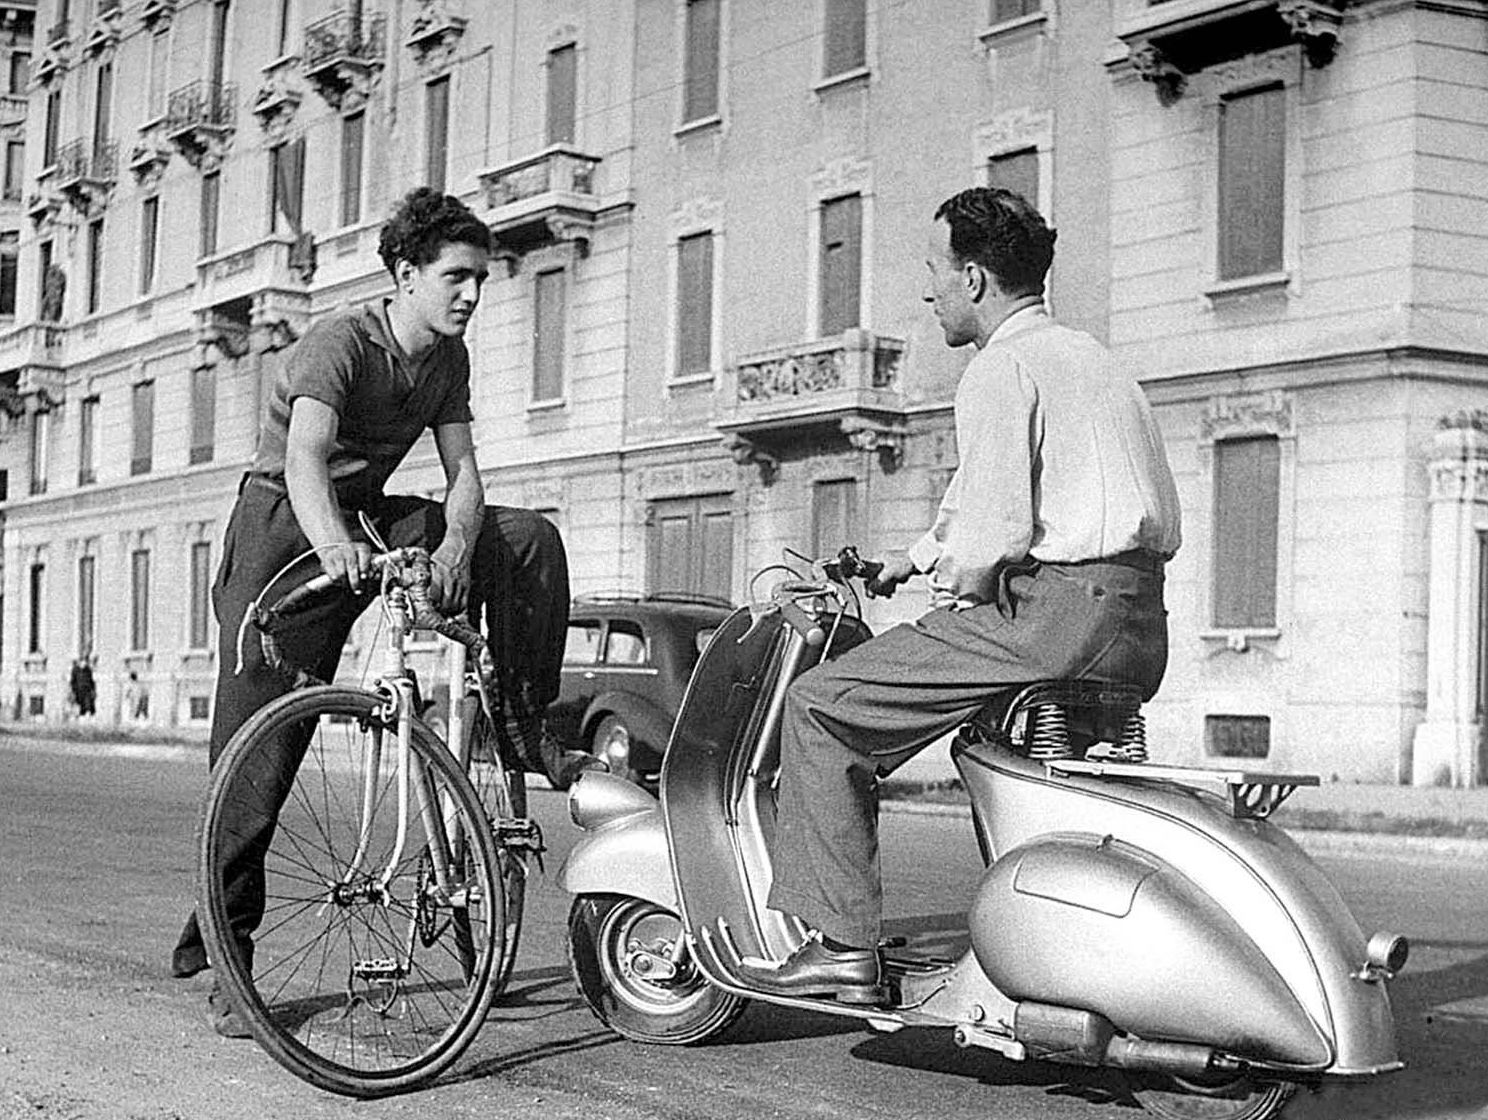
\includegraphics[width=.55\textwidth]{images/man_sitting_on_a_vespa_in_milan.jpg}};
			\node[below=0.2of pic] (cap)  {{\color{red}\underline{Man}} sitting on a
				{\color{blue}\underline{Vespa}}, \underline{Milan}, \underline{Italy} - \underline{1948}};
			\draw[thick,yellow] (-2.6,-2.1) rectangle (-.7,1.7);
			\draw[thick,red] (-.2,-2.1) rectangle (2,1.7);
			\draw[thick,green] (-2.4,-2.4) rectangle (-1,.1);
			\draw[thick,blue] (-.8,-2.5) rectangle (3.2,0);
			\draw[thick,orange] (-3.3,-1) rectangle (3.3,2.5);
			\end{tikzpicture}
		\end{center}
		\caption{\label{fig:ex_document} A complex document composed of a
			picture and a small text, annotated with visual and textual mentions.}
	\end{figure}
	Let us consider a knowledge base (e.g., YAGO \cite{yago}) that
	contains knowledge about the named entities $e_{\textit{Vespa}}$,
	$e_{\textit{Milan}}$, $e_{\textit{Italy}}$ and $e_{\textit{1948}}$ for
	``Vespa'', ``Milan'', ``Italy'' and ``1948'' respectivel, with the
	respective YAGO types
	${\textit{scooter}}$($e_{\textit{Vespa}}$),
	${\textit{town}}$($e_{\textit{Milan}}$),
	${\textit{country}}$($e_{\textit{Italy}}$), and
	${\textit{year}}$($e_{\textit{1948}}$). Let us suppose that the
	knowledge base contains also the concepts $\textit{man}$, and
	$\textit{building}$, and that we focus only on the these mentioned
	concepts.
	
	The solution of the VTKEL tasks requires (i) detecting the visual and
	textual entity mentions of the considered types, and linking them to
	either (ii) the correct, existing, named entities, or (iii) newly
	created entities, adding the corresponding type assertions.
	
	The visual and textual mentions of a man shown in the red text and in
	the red box refer 
	to the same entity, and they should be linked together. The other visual
	mention of a man, should be linked to another different entity. These two
	entities are not known (i.e., they are not part of the initial
	knowledge base $K$), and therefore two new entities of type man
	should be added to the knowledge base, i.e., the A-box of $K$ should
	be extended with the assertions $Man(e^{new}_1)$ and $Man(e^{new}_2)$.
	The textual and visual mentions of Vespa are also referring to the same
	entity. However, this time the entity is known (i.e., YAGO contains an
	entity for Vespa) and  therefore the two mentions should be linked
	to the same entity.%
	\footnote{Notice that here, for simplicity we don't take into account
		the fact that Vespa is a brand and the two mentions are not
		referring to the brand but to an instance of scooter of this
		brand. This issue, while surely important, is somehow not central to the
		main message of the paper, and considering it will make the
		presentation unnecessarily complex: therefore, we decide to ignore
		it at the moment.}
	The other visual mentions should be linked to new entities, with the
	correct type, i.e., we should add the assertions $bicycle(e^{new}_3)$,
	$building(e^{new}_4)$. For the other textual mentions, i.e., {\it Milan},
	{\it Italy}, {\it 1948},  we already have instances in the knowledge base, so we
	have to link them to these entities. 
\end{example}

VTKEL is a complex task that requires the solution of a set of well
studied elementary tasks in natural language processing and computer
vision. In particular, the following are the key subtasks of VTKEL:
\begin{itemize}
	\item (named) entity recognition and classification (i.e. typing) in texts \cite{goyal2018recent};
	\item object detection in images \cite{han2018advanced};
	\item textual co-reference resolution  \cite{sukthanker2018anaphora};
	\item textual entity linking to a knowledge base (ontology)\cite{shen2015entity};
	\item visual entity linking to a knowledge base (ontology) \cite{tilak2017visual};
	\item visual and textual co-reference resolution \cite{KongCVPR14,huang2017unsupervised,karpathy2015deep}.
\end{itemize}
In the recent literature, a number of approaches focusing on one
specific task, or a subset of them, can be found.  However, nowadays
it is well-established in many areas of NLP and computer vision (see
related work) that there is a clear advantage in solving complex tasks
in a collective/joint manner, rather than combining the results of
task-specific tools used as black-box It is indeed clear that the
relation among the appearance of an entity in an image, its associated
linguistic properties within the text, and the semantic/axiomatic
knowledge contained in the ontology, can jointly contribute to the
solution of the complex task altogether. We are particularly
interested in pursuing this research direction, and for this reason we
need to develop a dataset which is annotated with all the ground truth
data needed for the VTKEL problem.



%%%%%%%%%%%%%end of VTKEL task
\section{Related work}
\label{sec:related_work}

% As clarified in the introduction, the current paper has two main
% contributions. From the one hand it introduces the complex task of
% Visual-Textual-Knowledge Entity Linking, and on the other hand it
% proposes a fully annotated dataset for this task.

Recently the scientific community of NLP and IP devoted a reasonable
effort in investigating the interaction and integration of text and
image processing.  For a survery of the area of entity information
extraction and linking, we refer the reader to
\cite{martinez2018information}, which provides an up-to-date and
rather exhaustive survey of the approaches in the area.  In
particular: \cite{KongCVPR14} exploits natural language descriptions
of a picture in order to understand the content of the scene itself. 
the proposed approach solves the image-to-text coreference problem. 
It successively exploits visual information and visual-textual
coreference previously found to solve the coreference in text.
The work described in
\cite{weiland2017using,weiland2018knowledge}
tackle the problem of ranking the concepts from the knowledge base that
best represent the core message expressed in an image. This work
involves the three elements: Image, Text, and Knowledge, but it does
not provide information about the entities mentioned in the text and
shown in the image.  The approach in \cite{venkitasubramanian2017entity}
adopts a statistical model based on Markov Random Fields to represent
the dependencies between what is shown in a video frame and its
subtitle, and it is applied in the domain of video about wild-life animal. The main objective is
to detect the animal shown in a frame, and the mentions of animal
in the subtitle. The set of entities are the animal
names available in WordNet~\cite{wordnet}. Object detection is not
performed: the approach assumes that only one animal is shown in a
frame, and the vision part consists in image
classification. Furthermore, no background knowledge about animals is
used.  \cite{tilak2017visual} proposes a basic framework for visual
entity linking to DBpedia and Freebase. 
The approach involves also textual processing since the link of bounding boxes
to DBpedia and Freebase entities is found passing through an automatically
generated textual description of the image. The approach uses the Flickr8k dataset,
which is a subset of the Flikr30k-Entities dataset considered in our work.
\cite{ramanathan2014linking} combines textual coreference resolution with 
the linking of image and textual mentions in order to solve the problem
of assigning names of the people of the cast of a TV-show to the tracks of human
in the video, leveraging the screenplay scripts accompanying the video as a sort of 
raw supervision about who's in the video.

Concerning datasets that combine text and images, there are several
resources available. However, none of them has all the three
components necesary for the VTKEL
task. VisualGenome~\cite{krishnavisualgenome} is an extremely large
dataset that contains pictures in which objects are annotated along
with their types, attributes, and relationships. Each annotation is mapped to
some WordNet synset. Objects can also be annotated with some short sentence that
describes some qualitative property of the object.  E.g., ``The girl is feeding the
elephant'' or ``a handle of bananas''. However, there is no alignment
between the objects mentioned in these phrases and the objects shown in
the picture. E.g., there is no bounding box for the object ``bananas'' or
``elephant''.  The Visual Relationship Dataset
(VRD)~\cite{lu2016visual} is a dataset of images annotated with
bounding boxes around key objects. Furthermore, VRD contains
annotations about relationships between objects in the form of triplets
$\left<\mbox{object\_type},\mbox{relation},\mbox{subject\_type}\right>$
describing the scene. Examples of annotations are
$\left<man,riding,bicycle\right>$ and $\left<car,on,road\right>$.
However, these annotations are not aligned to any knowledge base. The
Microsoft COCO dataset~\cite{lin2014microsoft} contains pictures associated
with five captions.  They are annotated with objects regions of any
shape (not simple bounding boxes) and each
region is assigned with an object-type. This dataset does not contain
any information about 
relation between object regions, and relation between regions and
mentions in the captions.  Conceptual Captions~\cite{sharma2018conceptual} is a
recently introduced dataset that has been developed for automatic image
caption generation. It contains one order of magnitude more items 
than Microsoft COCO. It is a realistic dataset as images with
captions have been automatically extracted and filtered from the
web. However, there is no visual/textual mention annotation and
visual textual entity linking.  From the above analysis, it becomes clear that 
there is no dataset fully annotated with all the informations needed for
the VTKEL task. This justifies the development of such a new resource.


%%%%%end of related work
\section{Background} \label{sec:background}

To build the VTKEL dataset, we start from Flickr30k-Entities dataset \cite{plummer2015flickr30k}.  Flickr30K Entities provide the annotation of coreference chains, i.e., linking mentions of the same entities across different captions for the same image, and associating them with 276k manually annotated bounding boxes. Such annotations are essential for continued progress in automatic image description and grounded language understanding. They enable us to define a new benchmark for the localization of textual entity mentions in an image. To link textual entities to ontological resource, namely YAGO, we use PIKES~\cite{corcoglioniti2016frame}. In the following, we summarize these three main components.

\paragraph{Flickr30k-Entities - a dataset with visual and textual mentions
	alignment} The Flickr30k-Entities dataset~\cite{plummer2015flickr30k} has
become a standard benchmark for sentence-based image description tasks
such as image captioning. Flickr30k Entities has augmented the
original captions from Flickr30k-Entities with co-reference chains linking
mentions of the same entities in images, as well as manually annotated
bounding boxes corresponding to each entity. These additional
annotations are essential for grounded language understanding of
visual data, and they have allowed the recent progress in
text-to-image reference resolution and bidirectional image-sentence
retrieval. The availability of such ground-truth annotations is also a
key resource for experimenting in other high-level tasks, involving
both visual and textual data, such as Visual Question Answering (VQA).

\paragraph{YAGO - a large-scale semantic knowledge base}
YAGO\footnote{\url{http://yago-knowledge.org}}~\cite{yago} is a
large-scale semantic knowledge base automatically derived from several
data sources, including
Wikipedia,\footnote{\url{https://www.wikipedia.org/}}
WordNet,\footnote{\url{https://wordnet.princeton.edu/}} and
GeoNames.\footnote{\url{https://www.geonames.org/}} In particularly,
in YAGO an entity (e.g., person, organization, city, etc.) is
associated to its corresponding page in Wikipedia, and facts about the entity are
extracted from the infobox this Wikipedia page.
YAGO entities are typed according to classes organized in a class/sub-class
hierarchy obtained combining the categories of Wikipedia with the
WordNet synset taxonomy. The current version (v3) of YAGO contains
more than 350K classes and 17M entities, with over 150M facts about
them.

\paragraph{PIKES - A textual knowledge extraction suite}\
PIKES~\cite{corcoglioniti2016frame} is a state-of-the-art frame-based
framework for extracting knowledge (graphs) from natural language
text. It works in two phases. In the first \emph{linguistic feature
	extraction} phase, an RDF graph of mentions is obtained by running and
combining the outputs of several state-of-the-art NLP tools, including
Stanford
CoreNLP\footnote{\url{http://nlp.stanford.edu/software/corenlp.shtml}}
(tokenization, lemmatization, part-of-speech tagging, temporal
expression recognition and normalization, named entity recognition and
classification, coreference resolution, parsing), DBpedia
Spotlight\footnote{\url{http://spotlight.dbpedia.org/}} (entity
linking), UKB\footnote{\url{http://ixa2.si.ehu.es/ukb/}} (word sense
disambiguation),
Semafor\footnote{\url{http://www.cs.cmu.edu/~ark/SEMAFOR/}} and
Mate-tools\footnote{\url{http://code.google.com/p/mate-tools/}}
(semantic role labeling). In the second \emph{knowledge distillation}
phase, the mention graph is transformed into an RDF knowledge graph
through the evaluation of mapping rules, using the
RDFpro\footnote{\url{http://rdfpro.fbk.eu/}}~\cite{rdfpro2015sac} tool
for RDF processing. In particular, thanks to the DBpedia-YAGO and
WordNet-YAGO mappings, entities resulting in the final RDF knowledge
graph are typed according to the classes in YAGO. For the construction
of the VTKEL dataset, we run multiple instances of PIKES (using only
the minimal set of NLP tools needed for the purpose, namely Stanford
CoreNLP, DBpedia Spotlight, and UKB) on a server with 12 cores (24
threads) and 192 GB RAM, obtaining a throughput of
{\raise.17ex\hbox{$\scriptstyle\sim$}}3500K tokens/h.


%%%%  end of background
\section{VTKEL dataset and task}

%%%%  end of VKTEL dataset

\section{Baseline framework for VTKEL}
start here:ny full-width figures or tables (see the guidelines in
Subsection~\ref{ssec:first}). {\bf Type single-spaced.}  Start all


%%%% end of baseline
\section{Experiments and Evaluations of VTKEL}
start here:ny full-width figures or tables (see the guidelines in
Subsection~\ref{ssec:first}). {\bf Type single-spaced.}  Start all


\begin{table}[t!]
\begin{center}
\begin{tabular}{|l|rl|}
\hline \bf Type of Text & \bf Font Size & \bf Style \\ \hline
paper title & 15 pt & bold \\
author names & 12 pt & bold \\
author affiliation & 12 pt & \\
the word ``Abstract'' & 12 pt & bold \\
section titles & 12 pt & bold \\
document text & 11 pt  &\\
captions & 10 pt & \\
abstract text & 10 pt & \\
bibliography & 10 pt & \\
footnotes & 9 pt & \\
\hline
\end{tabular}
\end{center}
\caption{\label{font-table} Font guide. }
\end{table}

\begin{table}
\centering
\small
\begin{tabular}{cc}
\begin{tabular}{|l|l|}
\hline
{\bf Command} & {\bf Output}\\\hline
\verb|{\"a}| & {\"a} \\
\verb|{\^e}| & {\^e} \\
\verb|{\`i}| & {\`i} \\ 
\verb|{\.I}| & {\.I} \\ 
\verb|{\o}| & {\o} \\
\verb|{\'u}| & {\'u}  \\ 
\verb|{\aa}| & {\aa}  \\\hline
\end{tabular} & 
\begin{tabular}{|l|l|}
\hline
{\bf Command} & {\bf  Output}\\\hline
\verb|{\c c}| & {\c c} \\ 
\verb|{\u g}| & {\u g} \\ 
\verb|{\l}| & {\l} \\ 
\verb|{\~n}| & {\~n} \\ 
\verb|{\H o}| & {\H o} \\ 
\verb|{\v r}| & {\v r} \\ 
\verb|{\ss}| & {\ss} \\\hline
\end{tabular}
\end{tabular}
\caption{Example commands for accented characters, to be used in, {\em e.g.}, \BibTeX\ names.}\label{tab:accents}
\end{table}

\subsection{Sections}

{\bf Headings}: Type 

\begin{table*}[t!]
\centering
\begin{tabular}{lll}
  output & natbib & previous \conforg{} style files\\
  \hline
  \citep{Gusfield:97} & \verb|\citep| & \verb|\cite| \\
  \citet{Gusfield:97} & \verb|\citet| & \verb|\newcite| \\
  \citeyearpar{Gusfield:97} & \verb|\citeyearpar| & \verb|\shortcite| \\
\end{tabular}
\caption{Citation commands supported by the style file.
  The citation style is based on the natbib package and
  supports all natbib citation commands.
  It also supports commands defined in previous \conforg{} style files
  for compatibility.
  }
\end{table*}

{\bf Citations}: Citations within the text appear in parentheses
as~\cite{Gusfield:97} or, if the author's name appears in the text
itself, as Gusfield~\shortcite{Gusfield:97}.
Using the provided \LaTeX\ style, the former is accomplished using
{\small\verb|\cite|} and the latter with {\small\verb|\shortcite|} or {\small\verb|\newcite|}. Collapse multiple citations as in~\cite{Gusfield:97,Aho:72}; this is accomplished with the provided style using commas within the {\small\verb|\cite|} command, {\em e.g.}, {\small\verb|\cite{Gusfield:97,Aho:72}|}. Append lowercase letters to the year in cases of ambiguities.  
 Treat double authors as
in~\cite{Aho:72}, but write as in~\cite{Chandra:81} when more than two
authors are involved. Collapse multiple citations as
in~\cite{Gusfield:97,Aho:72}. Also refrain from using full citations
as sentence constituents.

We suggest that instead of
\begin{quote}
  ``\cite{Gusfield:97} showed that ...''
\end{quote}
you use
\begin{quote}
``Gusfield \shortcite{Gusfield:97}   showed that ...''
\end{quote}

If you are using the provided \LaTeX{} and Bib\TeX{} style files, you
can use the command \verb|\citet| (cite in text)
to get ``author (year)'' citations.

If the Bib\TeX{} file contains DOI fields, the paper
title in the references section will appear as a hyperlink
to the DOI, using the hyperref \LaTeX{} package.
To disable the hyperref package, load the style file
with the \verb|nohyperref| option: \\{\small
\verb|\usepackage[nohyperref]{acl2018}|}


\textbf{Digital Object Identifiers}: As part of our work to make ACL
materials more widely used and cited outside of our discipline, ACL
has registered as a CrossRef member, as a registrant of Digital Object
Identifiers (DOIs), the standard for registering permanent URNs for
referencing scholarly materials. \conforg{} has \textbf{not} adopted the
ACL policy of requiring camera-ready references to contain the appropriate
  DOIs (or as a second resort, the hyperlinked ACL Anthology
  Identifier). But we certainly encourage you to use
  Bib\TeX\ records that contain DOI or URLs for any of the ACL
  materials that you reference. Appropriate records should be found
for most materials in the current ACL Anthology at
\url{http://aclanthology.info/}.

As examples, we cite \cite{P16-1001} to show you how papers with a DOI
will appear in the bibliography.  We cite \cite{C14-1001} to show how
papers without a DOI but with an ACL Anthology Identifier will appear
in the bibliography.  

\textbf{Anonymity:} As reviewing will be double-blind, the submitted
version of the papers should not include the authors' names and
affiliations. Furthermore, self-references that reveal the author's
identity, {\em e.g.},
\begin{quote}
``We previously showed \cite{Gusfield:97} ...''  
\end{quote}
should be avoided. Instead, use citations such as 
\begin{quote}
``\citeauthor{Gusfield:97} \shortcite{Gusfield:97}
previously showed ... ''
\end{quote}

See the \verb|\bibliography| commands near the end for more.

Provide as complete a citation as possible, using a consistent format,
such as the one for {\em Computational Linguistics\/} or the one in the 
{\em Publication Manual of the American 
Psychological Association\/}~\cite{APA:83}. Use of full names for
authors rather than initials is preferred. A list of abbreviations
for common computer science journals can be found in the ACM 
{\em Computing Reviews\/}~\cite{ACM:83}.

The \LaTeX{} and Bib\TeX{} style files provided roughly fit the
American Psychological Association format, allowing regular citations, 
short citations and multiple citations as described above.  

\begin{itemize}
\item Example citing an arxiv paper: \cite{rasooli-tetrault-2015}. 
\item Example article in journal citation: \cite{Ando2005}.
\item Example article in proceedings, with location: \cite{borsch2011}.
\item Example article in proceedings, without location: \cite{andrew2007scalable}.
\end{itemize}
See corresponding .bib file for further details.


\subsection{URLs}

URLs can be typeset using the \verb|\url| command. 

\subsection{Footnotes}

{\bf Footnotes}: \footnote{This is how a footnote should appear.} .\footnote{Note the line
separating the footnotes from the text.}

\subsection{Graphics}



\subsection{Accessibility}
\label{ssec:accessibility}


% Min: no longer used as of ACL 2018, following ACL exec's decision to
% remove this extra workflow that was not executed much.
% BEGIN: remove
%% \section{XML conversion and supported \LaTeX\ packages}

%% Following ACL 2014 we will also we will attempt to automatically convert 
%% your \LaTeX\ source files to publish papers in machine-readable 
%% XML with semantic markup in the ACL Anthology, in addition to the 
%% traditional PDF format.  This will allow us to create, over the next 
%% few years, a growing corpus of scientific text for our own future research, 
%% and picks up on recent initiatives on converting ACL papers from earlier 
%% years to XML. 

%% We encourage you to submit a ZIP file of your \LaTeX\ sources along
%% with the camera-ready version of your paper. We will then convert them
%% to XML automatically, using the LaTeXML tool
%% (\url{http://dlmf.nist.gov/LaTeXML}). LaTeXML has \emph{bindings} for
%% a number of \LaTeX\ packages, including the ACL 2018 stylefile. These
%% bindings allow LaTeXML to render the commands from these packages
%% correctly in XML. For best results, we encourage you to use the
%% packages that are officially supported by LaTeXML, listed at
%% \url{http://dlmf.nist.gov/LaTeXML/manual/included.bindings}
% END: remove

\section{VTKEL baseline framework}

It is also.

\section{Evaluation}
\label{sec:length}

The \confname{} main conference accepts submissions of long papers and
short papers.

 (see Appendix
\ref{sec:supplemental}). Papers that d


\section*{Conclusion and future work}

\section*{Acknowledgments}

The acknowledgments . \\

\noindent {\bf Preparing References:} \\

Include your own bib file like this:
{\small\verb|\bibliographystyle{acl_natbib_nourl}|
\verb|\bibliography{emnlp2018}|}

Where \verb|emnlp2018| corresponds to the {\tt emnlp2018.bib} file.
\bibliography{emnlp2018}
\bibliographystyle{acl_natbib_nourl}

\appendix

\section{Supplemental Material}
\label{sec:supplemental}
Each \confname{} submission can be accompanied by a single PDF
appendix, one {\small\tt.tgz} or {\small\tt.zip} appendix containing
software, and one {\small\tt.tgz} or {\small\tt.zip} appendix
containing data.

\confname{} also 


Appendices ({\em i.e.} supplementary material in the form of proofs, tables,
or pseudo-code) should be {\bf uploaded as supplementary material} when submitting the paper for review.
Upon acceptance, the appendices come after the references, as shown here. Use
\verb|\appendix| before any appendix section to switch the section
numbering over to letters.

\end{document}
